\section{Related Work}\label{sec:related_work}


\subsection{Handwriting Recognition} % remove if I'm out of space...

``In numerous situations, a pen together with paper or a small notepad is more convenient that a keyboard''\cite{handwriting_survey}.
Early research in automated recognition of handwriting was motivated by the desire to allow humans to write conveniently and then parse that writing into data inside of a computer.

``On-line'' systems do this given the 2-D coordinates of the writer's pen as a function of time.% and require writing to be captured live by special electronic devices.
``Off-line'' systems only need images of the handwriting, so they are more broadly applicable\cite{handwriting_survey}.

Personal Digital Assistants (PDAs) incorporating on-line systems have been widely used commercially.
These systems have used rule-based, statistical, and implicit methods\cite{handwriting_survey}, especially Hidden Markov Models and even convolutional neural networks\cite{389575} (while Yann LeCun's foundational work was in its early stages\cite{mnist}).

None of these methods have been accurate enough to be used commercially on cursive writing\cite{handwriting_survey}.
As of 2000, on-line handwriting recognition was more accurate than off-line recognition because the chronological information is useful\cite{handwriting_survey}.
% However, off-line handwriting recognition is much more broadly applicable because it does not require a special device to capture the handwriting.
% Only a camera is needed to capture an image of the writing.
There have been several attempts made to recreate the temporal data from an image, but these have not been very successful\cite{handwriting_survey}.

% A bank might require an error of 1/ 100,000. ``Current systems are sill several orders of magnitude away''.


\subsection{Contrastive Loss}\label{sec:contrastive_loss}

In 2005, Yann LeCun co-authored a paper that describes a technique for face verification.
It maps ``images of faces to points in a low dimensional space so that the distance between these points is small if the images belong to the same person and large otherwise''\cite{LeCun}.

% This can be done by training a classifier and then interpreting an intermediate layer to be a latent space, but this doesn't perform very well, even after performing principal component analysis on the output\cite{face_net}.

As seen in figure \ref{fig:siamese}, two identical CNNs (called siamese networks) that share weights both map images to the low dimensional (latent) space.
A ``contrastive loss'' function is then used to train the siamese networks.
This loss function penalizes distance between genuine pairs and encourages distance between impostor pairs (those where the images are of different people)\cite{LeCun}.
\begin{figure}[h]
    \begin{center}
        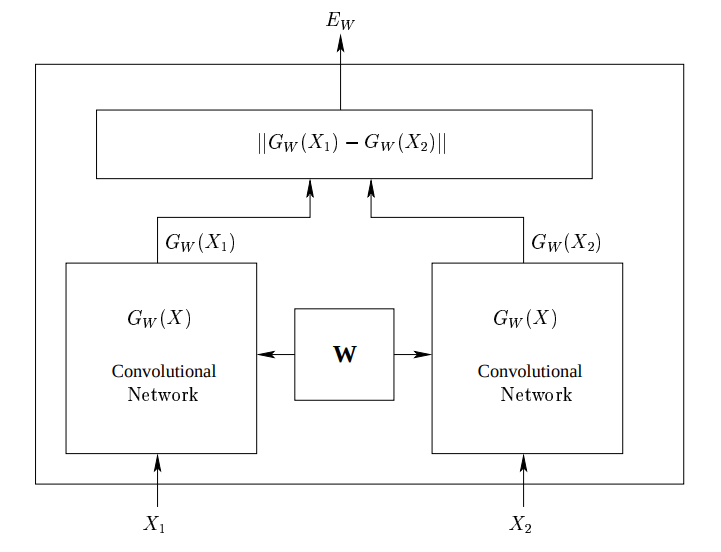
\includegraphics[width=0.8\linewidth]{siamese_architecture.png}
    \end{center}
    \caption{Siamese Architecture. (LeCun et al. 2005)}
    \label{fig:siamese}
\end{figure}
% [Note: the partitioning and pairing of images is the same idea as SigNet.]

The distribution of the latent vectors for images of each person is assumed to be Gaussian.
This distribution is computed for each person using the first five images of them.
Verification on a new image is performed by comparing the probability that the image's latent vector is genuine vs. an impostor given the Gaussian distribution for the given person\cite{LeCun}.


\subsection{FaceNet and Triplet Loss} % remove this if I run out of space

FaceNet (\cite{triple_loss}) presents ``triplet loss'', an alternative to contrastive loss that allows datapoints with the same label to live in multiple clusters without being penalized.
While training with contrastive loss operates on pairs of images, triplet loss uses two matching images and one impostor, and ``encourages a relative distance constraint''\cite{face_net}.

Using this loss function, FaceNet was built off of LeCun's work (discussed in section \ref{sec:contrastive_loss}) and achieved very impressive results\cite{face_net}.
Although FaceNet does aim for each person's latent vectors to be in one cluster, the creators ``believe that the triplet loss is more suitable for face verification'' because it allows images of one person to live on a manifold rather than being confined to a point in the latent space\cite{face_net}.

There are several other, more subtle differences between FaceNet and LeCun's work in 2005.
FaceNet does not consider true negatives when training because the network already knows the images are of different people, so it is not productive to adjust the weight of the network as the direction of the gradient is somewhat arbitrary.
% [Maybe I should try that...]

Instead of computing Gaussian distributions, a simple distance threshold is used for deciding if two latent vectors match.
(The paper does not seem to explain how the threshold is computed.)

The FaceNet creators also conclude from their experiments that using latent vectors larger than 128 dimensions does not result in significant improvements in model accuracy\cite{face_net}.
% say thing about being able to compress to 128 bytes?


\subsection{SigNet}\label{sec:sig_net}

SigNet is a siamese network similar to FaceNet that performs handwritten signature verification.
It uses contrastive loss and 128-dimensional latent vectors.

In the validation process, SigNet takes an image and outputs a latent vector.
First, a genuine signature is sent through the network.
Then, either another genuine or a forge is sent through the network.
The resulting latent vectors are compared using Euclidean distance.
% [have I described partitioning yet?]
After computing the latent vector distances for all image pairs in the validation set, the threshold that results in the best accuracy is picked.
This results in 100\% accuracy on the CEDAR dataset, which contains skilled forgeries.

The SigNet paper does not explain the decision to use contrastive loss over triplet loss.
Since signature verification is simpler than face verification (and SigNet is much smaller and was trained for far less time than FaceNet), is seems that contrastive loss was used because it is much simpler to implement and has fewer hyper-parameters\cite{sig_net}\cite{face_net}.


\subsection{FGSM}\label{sec:fgsm}

It is known that state-of-the-art deep neural networks are unstable to small, well sought, perturbations of their inputs\cite{deep_fool}.

Ian Goodfellow (famous for his development of generative adversarial networks) has proven that even linear models are susceptible to adversarial attacks consisting of minute perturbations if their dimensionality is large enough\cite{goodfellow}.

This is interesting in the topic of signature verification because adversarial attacks could pose a security threat if such verification systems were used in the future.

Fast Gradient Sign Method (FGSM) is a technique for generating adversarial inputs for models\cite{goodfellow}.
An existing input is sent through the model and then the gradient of the loss is taken with respect to the input.
The input is then perturbed in the opposite direction of the gradient by some distance epsilon.
This produces a new (perturbed) input that is very similar to the original, but produces a very different output.

They hypothesize that the reason that this works is that neural networks are designed to have some linear properties so that gradients can be computed, allowing the model to be trained\cite{goodfellow}. 

They also show that training on adversarial inputs improves the model's accuracy on adversarial inputs (making it less susceptible to the FGSM attack).

``An intriguing aspect of adversarial examples is that an example generated for one model is often
misclassified by other models, even when they have different architectures or were trained on disjoint training sets''\cite{goodfellow}.
% The paper also says that adversarial examples generalize to different instances and even different models... (it is really the direction of the pertebation that matters).

If a signature verification system were used (for cheques for example), an attacker could use FGSM without gaining access to the model or probing it.
If they have access to a similar training set to that used for training the system under attack, they could train their own model and find perturbations using FGSM on their model.

% `` However, noise
% with zero mean and zero covariance is very inefficient at preventing adversarial examples. The
% expected dot product between any reference vector and such a noise vector is zero. This means that
% in many cases the noise will have essentially no effect rather than yielding a more difficult input.''
% ...this means that adding my noise shouldn't really fool SigNet.

% [If I decide to do the test on different latent vector sizes, I definitely want to mention what Goodfellow says about higher dimensional spaces being the reason for perturbations allowing for FGSM attacks!]

% https://arxiv.org/pdf/1805.06605.pdf
% This talks about randomized FGSM, which applies a random perturbation and then FGSM.
